\documentclass[aspectratio=169,10pt]{beamer}
\usetheme{Madrid}
\usecolortheme{seahorse}
\setbeamertemplate{footline}[frame number]

\usepackage[utf8]{inputenc}
\usepackage{amsmath,amssymb,amsthm}
\usepackage{graphicx}
\usepackage{listings}
\usepackage{xcolor}
\usepackage{tikz}

\graphicspath{{figures/}}

\lstset{
  basicstyle=\ttfamily\scriptsize,
  numbers=left,
  frame=single,
  backgroundcolor=\color{gray!7},
  keywordstyle=\color{blue}\bfseries,
  commentstyle=\color{green!50!black}\itshape,
  stringstyle=\color{red!60!black},
  breaklines=true,
  showstringspaces=false,
  language=Python
}

\newcommand{\B}{\mathbb{B}}
\newcommand{\N}{\mathbb{N}}
\newcommand{\R}{\mathbb{R}}
\newcommand{\Z}{\mathbb{Z}}
\newcommand{\Q}{\mathbb{Q}}

\title{Background: Computability Theory}
\subtitle{Section 2.6}
\author{Chapter 2 --- Background}
\institute{An Introduction to Universal Artificial Intelligence \\ \small Hutter, Quarel, Catt (2024)}
\date{}

\begin{document}

% ============================================================
\begin{frame}
  \titlepage
\end{frame}

% ============================================================
\begin{frame}{Outline}
  \tableofcontents
\end{frame}

\section{What is an Algorithm?}

% ============================================================
\begin{frame}{Why We Need a Formal Notion of ``Algorithm''}
  Computability theory narrowly \textbf{predates computers themselves}: it was
  mainly introduced in Turing's 1936 paper. The idea of an \emph{algorithm} ---
  a well-defined, unambiguous sequence of steps that solves a problem --- has
  been known since antiquity.

  \begin{block}{Example: Euclid's algorithm}
    To compute the greatest common divisor of two numbers, break the computation
    into a sequence of steps (additions, comparisons) so simple that each step
    is obviously executable in a constant amount of time.
  \end{block}

  \textbf{The problem:} to even talk rigorously about ``what can be computed,''
  we must fix a formal language in which algorithms are written, together with
  an agreed reference set of allowed elementary operations. \textbf{Turing
  machines} provide exactly such a formalization.

  \vspace{2mm}
  We will build a \emph{hierarchy of computability}, measuring how well an
  algorithm can be written to solve a given problem: fully computable, only
  approximately computable, or not computable at all.
\end{frame}

% ============================================================
\begin{frame}{Definition: Decision Problems and Languages}
  \begin{block}{Definition 2.6.1 (Decision Problem and Language)}
    Given an alphabet $\Sigma$ (often $\B = \{0,1\}$), a \emph{decision problem}
    or \emph{language} $L$ over $\Sigma$ is a subset $L \subseteq \Sigma^{*}$.
  \end{block}

  \textbf{Plain English.} $\Sigma^{*}$ is the set of all finite strings you can
  write using the symbols (``letters'') of $\Sigma$. A decision problem is just
  a yes/no question about strings, encoded as: ``is this string $x$ a member of
  the set $L$?''

  \vspace{2mm}
  \textbf{Why this is not restrictive.} Any predicate (true/false statement)
  over $\Sigma^{*}$ can be encoded as such a set of strings for which the
  predicate is true. We can talk about predicates over other objects (natural
  numbers, vectors, graphs, \dots) by first encoding them as binary strings.
  Even computing a general function $f: \Sigma^{*} \to \Xi$ (for a finite
  output alphabet $\Xi$) reduces to solving decision problems: replace $\Xi$
  with $\B^{m}$ for suitable $m$, and set $P_i = \{x \in \Sigma^{*} : f(x)_i = 1\}$.
  Solving all the decision problems $(x \in P_1, \dots, x \in P_m)$ is
  equivalent to computing $f$.
\end{frame}

\section{2.6.1 Models of Computation}

% ============================================================
\begin{frame}{The Turing Machine: Intuition}
  Turing's chosen model of computation is the \textbf{Turing machine}. It has
  two parts:
  \begin{itemize}
    \item a \textbf{finite control}: a function describing the operation to
      perform, plus a finite collection of \emph{states} it can be in;
    \item a \textbf{tape}: a one-dimensional grid of cells extending infinitely
      in both directions, each cell holding one symbol from a finite alphabet.
  \end{itemize}
  A \textbf{head} reads/writes the current cell and moves one step left or
  right. The input is placed on the tape, other cells hold a reserved
  \emph{blank} symbol $B$, and the head starts on the left-most input cell.

  \textbf{How it runs.} At each time step $t=1,2,\dots$, the machine reads the
  symbol under the head and its current state, then writes a new symbol,
  moves to a new state, and moves the head left ($L$) or right ($R$).

  \begin{center}
    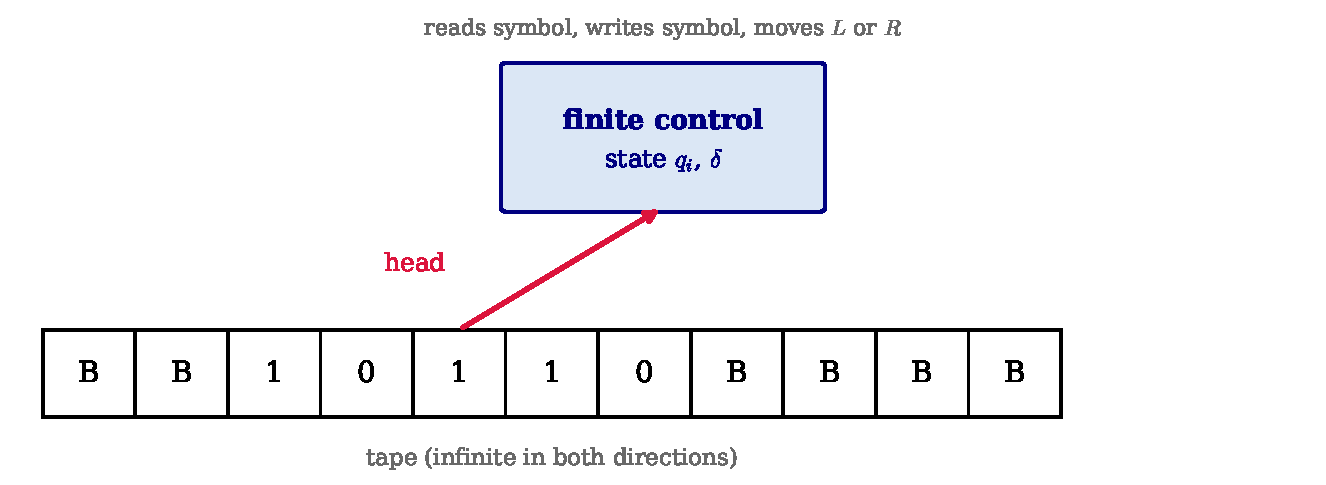
\includegraphics[width=0.58\textwidth]{turing_machine}
  \end{center}
\end{frame}

% ============================================================
\begin{frame}[allowframebreaks]{Formal Definition of a Turing Machine}
  \begin{block}{Definition 2.6.2 (Turing Machine)}
    A Turing machine (TM) is a 7-tuple $T = (Q, \Sigma, \Gamma, \delta, q_0, B, F)$
    where:
    \begin{itemize}
      \item $Q = \{q_0, q_1, \dots, q_n\}$ is a finite set of \emph{states}.
      \item $\Sigma$ is a finite set of input symbols, called the
        \emph{alphabet} (usually $\Sigma = \B$).
      \item $\Gamma$ is a finite set of tape symbols with $\Sigma \subseteq \Gamma$.
      \item $\delta$ is a partial function
        $\delta : Q \times \Gamma \to Q \times \Gamma \times \{L, R\}$, the
        \emph{(partial) transition function}. It takes the current state and
        the symbol under the read head, and returns a new state, a new symbol
        to write, and a direction ($L$ or $R$) to move the head.
      \item $q_0 \in Q$ is the \emph{start state}.
      \item $B \in \Gamma \setminus \Sigma$ is the reserved \emph{blank symbol}
        pre-filling the tape.
      \item $F \subseteq Q$ is the set of \emph{final} or \emph{accepting}
        states.
    \end{itemize}
  \end{block}

  \textbf{Plain English, symbol by symbol.} $Q$ is the machine's ``memory of
  mode'' --- like a light switch with finitely many positions. $\Sigma$ is the
  alphabet the input is written in; $\Gamma$ may include extra ``scratch''
  symbols beyond $\Sigma$. $\delta$ is the rulebook: given (state, symbol
  read), it tells you (new state, symbol to write, which way to move). If
  $\delta$ is undefined on the current (state, symbol) pair, the machine
  \emph{halts} --- it simply stops. $q_0$ is where execution begins, $B$ marks
  ``nothing written here,'' and $F$ marks the states in which halting counts as
  ``accept.''

  \framebreak

  \textbf{Why bother with something this low-level?} Writing complex algorithms
  directly as a Turing machine is as laborious as writing machine code by hand
  instead of using a high-level programming language. But it gives us a fixed,
  theoretically clean reference machine for reasoning about \emph{what can be
  computed at all} --- independent of any particular programming language.

  We can view the action of a Turing machine in two equivalent ways: as a
  \emph{predicate} on strings (does it accept or reject?), or as a
  \emph{function} from strings to strings (what does it output?).

  \begin{block}{Definition 2.6.3 (Language of a TM)}
    Given a TM $T$, the \emph{language} of $T$, denoted $L(T)$, is the set of
    all strings $x$ such that running $T$ with the tape initialized to $x$
    causes $T$ to halt in an accepting state:
    \[
      L(T) := \{ x \in \Sigma^{*} : T(x) \text{ halts and accepts} \}.
    \]
  \end{block}
  \textbf{Plain English.} $L(T)$ collects exactly the inputs that $T$ says
  ``yes'' to (and halts while saying it).

  \begin{block}{Definition 2.6.4 (Behavior of a TM)}
    Given a TM $T$, we write $T(x) = y$ if $T$ halts with $y$ on the tape when
    started with $x$ on the tape. If $T$ does not halt on input $x$, we write
    $T(x) = \bot := \text{undefined}$.
  \end{block}
  \textbf{Plain English.} $T(x)$ is simply ``the output of running program $T$
  on input $x$'' --- and $\bot$ (bot) is the symbol we use when the program
  never finishes, so it has no output.
\end{frame}

% ============================================================
\begin{frame}{Partial Recursive Functions and the Church--Turing Thesis}
  \begin{block}{Definition 2.6.5 (Partial Recursive Functions)}
    A function $f : \Sigma^{*} \to \Xi^{*} \cup \{\bot\}$ is called
    \emph{partial recursive} if it is computable by a Turing machine $T$
    (with $\Gamma \supseteq \Sigma \cup \Xi$), i.e.\ if
    $\exists T.\; f(x) = T(x)\; \forall x$.
  \end{block}
  \textbf{Plain English.} ``Partial recursive'' is just formal jargon for
  ``there is some Turing machine that computes exactly this function'' (and it
  is allowed to not halt --- i.e.\ be undefined --- on some inputs).

  \vspace{2mm}
  Turing found that many familiar algorithms (viewed as functions from strings
  to strings) can be implemented by designing a suitable Turing machine. This
  led to a bold claim, stated next.
\end{frame}

% ============================================================
\begin{frame}{The Church--Turing Thesis}
  \begin{block}{Thesis 2.6.6 (Church--Turing Thesis)}
    \textbf{Church:} The class of algorithmically computable numerical
    functions (in the intuitive, informal sense) coincides with the class of
    partial recursive functions. \\[1mm]
    \textbf{Turing:} Everything that can be reasonably said to be computable by
    a human using a fixed procedure can also be computed by a Turing machine.
  \end{block}
  \textbf{Plain English.} This is a \emph{thesis}, not a theorem, because
  ``computable in the intuitive sense'' and ``computable by a human'' are
  informal, not formally defined notions. It is a claim about matching an
  informal idea to a formal one --- and it has held up since 1936 against
  every alternative formalization anyone has proposed.
\end{frame}

% ============================================================
\begin{frame}{Alternative Formalizations: General Recursive Functions}
  Gödel and Herbrand proposed a different route to the same destination,
  starting from a small set of \emph{primitive functions}:
  \begin{itemize}
    \item the \textbf{constant} function (of arbitrary arity),
    \item the unary \textbf{successor} function,
    \item the \textbf{projection} function (returns one of the $n$ input
      arguments).
  \end{itemize}
  They then define three \textbf{operators} that build new functions out of
  old ones:
  \begin{itemize}
    \item \textbf{Composition}: chain functions together.
    \item \textbf{Recursion}: a function may call itself (or another function)
      several times.
    \item \textbf{Minimization}: given an $(n+1)$-ary function $f$ and
      arguments $x_1,\dots,x_n$, return the smallest $z$ such that
      $f(z, x_1,\dots,x_n) = 0$ and $f(z', x_1,\dots,x_n)$ is defined for
      every $z' < z$.
  \end{itemize}
  \textbf{Plain English.} You start from a handful of trivial building blocks
  and glue them together with these three operators. The closure of the
  primitive functions under composition, recursion, and minimization is called
  the class of \emph{general} (or \emph{partial recursive}) functions --- and
  it was proposed as another formal candidate definition for ``algorithmically
  computable.''
\end{frame}

% ============================================================
\begin{frame}{Alternative Formalizations: Lambda Calculus}
  Alonzo Church's \emph{lambda calculus} ($\lambda$-calculus) is, at face
  value, much simpler than general recursive functions --- its definition fits
  in one line. Fix a set of variables $V = \{x, y, z, \dots\}$. Every lambda
  expression $e$ has one of three forms:
  \[
    e \; := \; v \mid \lambda v.e_1 \mid e_1 e_2
  \]
  \textbf{Plain English, term by term.} $v$ is a bare \emph{variable}.
  $\lambda v.e_1$ \emph{abstracts} $e_1$ by the variable $v$ --- think of it as
  ``a function of $v$ that returns $e_1$.'' $e_1 e_2$ \emph{applies} expression
  $e_1$ (thought of as a function) to the argument $e_2$. Every lambda
  expression is one of: a variable, an abstraction, or an application.

  \vspace{2mm}
  Only two operations act on these expressions:
  \begin{itemize}
    \item $\alpha$-conversion (alpha): renaming variables bound to a $\lambda$
      quantifier, to avoid name collisions.
    \item $\beta$-reduction (beta): substituting an abstracted variable for the
      expression it is applied to (i.e.\ actually ``running'' the function).
  \end{itemize}
  \textbf{Remarkably}, these minimal rules suffice to define the natural
  numbers and arithmetic on them (addition, multiplication, equality) purely
  within lambda calculus; higher-level concepts can then be built on top.
\end{frame}

% ============================================================
\begin{frame}{Turing Completeness and the Choice of Model}
  We now have (at least) three candidate definitions of ``algorithmically
  computable'': Turing's Turing machines, Church's lambda calculus, and
  Gödel/Herbrand's general recursive functions. As it turns out, \textbf{all
  of these end up equivalent} --- they define exactly the same class of
  functions.

  \begin{block}{Turing Completeness}
    A model of computation (or formal system) is called \emph{Turing complete}
    if it is at least as expressive as a Turing machine: any algorithm
    implementable by a Turing machine can also be implemented within that
    model. In practice this is usually shown by emulating a \emph{universal}
    Turing machine within the system.
  \end{block}

  Many other systems --- often designed for entirely different purposes ---
  have later been discovered to be Turing complete. A striking example:
  \textbf{cellular automata}, an infinite grid of cells, each in one of
  finitely many states, updated by a rule depending on neighboring cells.
  Conway's \emph{Game of Life} and the one-dimensional \emph{Rule 110} both
  exhibit starkly complex behavior despite trivially simple rules --- and both
  turn out to be Turing complete.

  \vspace{2mm}
  \textbf{Consequence.} Since the choice of model does not matter, this book
  sticks with Turing machines by convention, but freely appeals to the
  Church--Turing thesis and to modern (Turing complete) programming languages
  instead of explicitly constructing Turing machines.
\end{frame}

% ============================================================
\begin{frame}[fragile]{Python: Simulating a Turing Machine}
  A tiny Turing machine: scan right over a block of \texttt{1}s on a binary
  tape, then add one more \texttt{1} at the end (unary increment) and halt.
  This is a partial recursive function computed step by step, as in
  Definition 2.6.2. States: \texttt{q0} (scan right), \texttt{qw} (write
  extra 1), \texttt{qh} (halt).
\begin{lstlisting}
def run_tm(tape, head=0, state='q0', max_steps=200):
    tape = dict(enumerate(tape))                     # sparse infinite tape
    for step in range(max_steps):
        sym = tape.get(head, 'B')
        if state == 'q0':
            state, write, move = ('q0','1',1) if sym == '1' else ('qw','1',1)
        elif state == 'qw':
            state, write, move = 'qh', sym, 0        # accept & halt
        tape[head] = write; head += move
        if state == 'qh': break
    lo, hi = min(tape), max(tape)
    return ''.join(tape.get(i, 'B') for i in range(lo, hi + 1)), step + 1

output, steps = run_tm(list("111"))
print(output, steps)          # -> '1111' 4  (three 1's become four 1's)
\end{lstlisting}
  \textbf{Plain English.} $T(\texttt{111}) = \texttt{1111}$: the first blank
  cell tells the machine the number has ended, so it writes one extra
  \texttt{1} and halts --- exactly the function ``add one,'' in unary.
\end{frame}

\section{2.6.2 The Halting Problem}

% ============================================================
\begin{frame}{From Hilbert's Program to Gödel's Incompleteness Theorem}
  In 1900, David Hilbert posed a list of the most pressing open problems of
  mathematics. In \emph{zeroth-order logic} (propositional logic), statements
  are built only from Boolean variables and connectives ($\land, \lor, \neg$);
  since each variable is Boolean-valued, we can brute-force all $2^{n}$
  assignments to check whether an $n$-variable statement is \emph{valid} (true
  under every assignment).

  \emph{First-order logic} additionally allows \textbf{quantifiers}
  ($\exists$ and $\forall$, pronounced ``there exists'' and ``for all''). If
  the domain of a predicate is infinite (e.g.\ the natural numbers), naively
  checking every value is no longer possible. Hilbert asked: does an algorithm
  exist that can verify the validity of \emph{every} first-order logic
  statement?
\end{frame}

% ============================================================
\begin{frame}{G\"odel Incompleteness}
  \begin{block}{Gödel Incompleteness}
    The answer is \textbf{no}. Gödel's incompleteness theorem shows that any
    sufficiently powerful formal system (capable of a certain amount of
    arithmetic) that is \emph{consistent} (cannot prove contradictions) must
    contain statements that are true, but that cannot be proven true within
    the system itself.
  \end{block}

  \textbf{The proof idea.} Construct the self-referential
  \emph{Gödel statement} $G := $ ``$G$ cannot be formally proven,'' and encode
  this statement as a number, so the system can (indirectly) state predicates
  about itself. Within the theory, $G$ cannot be proven; but reasoning
  \emph{outside} the formal system shows $G$ is in fact true. (If $G$ were
  provable it would assert its own unprovability --- a contradiction; if $G$
  were false, it would say it is provable, hence true --- also a
  contradiction. So $G$ must be true.)
\end{frame}

% ============================================================
\begin{frame}{Why Care? The Halting Problem}
  As a corollary of incompleteness, there must be problems that not even a
  Turing machine can hope to solve. The canonical example: the
  \textbf{Halting Problem}.

  \textbf{Motivation.} When we write programs, it is often unclear whether
  they will run forever or eventually stop. An algorithm that could decide
  this in general would be extremely useful --- and dangerously powerful. For
  instance, the Goldbach conjecture (every even $n \geq 4$ is the sum of two
  primes) could be resolved by a program that searches for counterexamples and
  halts if one is found; the conjecture is true if and only if that program
  never halts. If a universal halting-decider existed, many open problems in
  mathematics would become trivial to settle --- which is a strong hint that
  no such algorithm can exist.

  \vspace{2mm}
  \textbf{Setup.} Assume a canonical encoding of Turing machines as binary
  strings, and the ability to encode tuples (pairs, triples, \dots) as a
  single string so that the components can be recovered (e.g.\ via a prefix
  code). This lets a Turing machine take the encoding of \emph{another} Turing
  machine as input, feeding one machine's binary description onto the tape of
  another.
\end{frame}

% ============================================================
\begin{frame}{Theorem: The Halting Problem is Undecidable}
  \begin{block}{Theorem 2.6.7 (Halting Problem)}
    Let $L_H = \{ (\langle M \rangle, w) : M(w) \text{ halts} \}$ denote the
    \emph{halting language}: the set of all pairs of (an encoded Turing
    machine $M$, a string $w$) such that running $M$ on $w$ halts. Then there
    exists no Turing machine $T$ that halts on all inputs and has
    $L(T) = L_H$.
  \end{block}
  \textbf{Plain English.} $\langle M \rangle$ (angle brackets) denotes ``the
  binary encoding of machine $M$.'' $L_H$ is the set of all (program,
  input) pairs where the program eventually stops. The theorem says: there is
  \emph{no} program $T$ that always halts and always correctly answers ``does
  $M$ halt on $w$?'' --- a universal ``will this program terminate?''
  detector is mathematically impossible.

  \vspace{2mm}
  \textbf{Proof strategy (by contradiction).} Assume such a $T$ exists. Using
  $T$ as a subroutine, build a new machine $P$ that does the \emph{opposite} of
  what $T$ predicts about a program run on \emph{its own} description --- and
  then feed $P$ its own description. Whatever happens next contradicts what
  $T$ was assumed to correctly predict.
\end{frame}

% ============================================================
\begin{frame}{Proof of the Halting Problem, Part 1: The Construction}
  Assume, for contradiction, that a total (always-halting) Turing machine $T$
  exists with $L(T) = L_H$. Given $T$, construct a new machine $P$ that, on
  input $\langle M \rangle$ (an encoded machine), performs:
  \[
    P(\langle M \rangle) \;=\;
    \begin{cases}
      \bot & \text{if } T(\langle M \rangle, \langle M \rangle) \text{ accepts} \\
      1 & \text{if } T(\langle M \rangle, \langle M \rangle) \text{ rejects}
    \end{cases}
  \]
  \textbf{Plain English.} $P$ feeds $M$'s own description to itself (as both
  ``the program'' and ``the input''), and asks the hypothetical halting oracle
  $T$: ``does $M(M)$ halt?'' If $T$ says \emph{yes} (accepts), $P$
  deliberately loops forever ($\bot$); if $T$ says \emph{no} (rejects), $P$
  halts and outputs $1$. That is: $P$ is built to always do the opposite of
  what $T$ predicts $M(M)$ would do.

  \vspace{2mm}
  Since $P$ is itself just a Turing machine (built out of $T$ plus this extra
  logic), it has some binary encoding $\langle P \rangle$. The key trick: what
  happens if we run $P$ on \emph{its own} encoding, i.e.\ compute
  $P(\langle P \rangle)$? Either it must run forever, or it must halt.
\end{frame}

% ============================================================
\begin{frame}{Proof of the Halting Problem, Part 2: The Contradiction}
  \begin{itemize}
    \item \textbf{Case A: suppose $P(\langle P \rangle)$ halts.} By
      construction of $P$, this means $T(\langle P \rangle, \langle P \rangle)$
      must have \emph{rejected} (that is the only branch of $P$ that halts).
      So $(\langle P \rangle, \langle P \rangle) \notin L_H$ --- meaning
      $P(\langle P \rangle)$ should \emph{not} halt. Contradiction.
    \item \textbf{Case B: suppose $P(\langle P \rangle)$ runs forever.} By
      construction of $P$, this means $T(\langle P \rangle, \langle P \rangle)$
      must have \emph{accepted} (that is the only branch of $P$ that loops).
      So $(\langle P \rangle, \langle P \rangle) \in L_H$ --- meaning
      $P(\langle P \rangle)$ should halt. Contradiction.
  \end{itemize}

  \vspace{3mm}
  \textbf{In either case we get a contradiction}, so our assumption --- that a
  total $T$ deciding $L_H$ exists --- must be false. \hfill $\blacksquare$

  \vspace{3mm}
  \textbf{Why this matters.} Even with \emph{no} constraints on memory or time
  allotted, no Turing machine can solve all problems. This motivates a whole
  hierarchy of ``how computable'' a set or function is, since perfect
  computability is simply out of reach for many interesting problems.
\end{frame}

% ============================================================
\begin{frame}{Recursive and Recursively Enumerable Sets}
  \begin{block}{Definition 2.6.8 (Recursive / Recursively Enumerable)}
    A language or set $S$ is \emph{recursive} if there exists a
    \emph{total} Turing machine $T$ (one that halts on all inputs) such that
    $L(T) = S$. We say $S$ is \emph{recursively enumerable} (RE) if we drop the
    requirement that $T$ be total (i.e.\ $T$ may loop forever on non-members).

    Similarly, a partial function $f$ is \emph{recursive} (resp.\
    \emph{recursively enumerable}) if there is a total TM (resp.\ partial TM)
    $T$ such that $f(x) = y \iff T(x) = y$.
  \end{block}
  \textbf{Plain English.} ``Recursive'' = \emph{decidable}: there is a program
  that always halts and correctly says yes/no for every input --- this is
  often just called \textbf{computable} in the context of decision problems.
  ``Recursively enumerable'' is weaker: there is a program that halts and says
  \emph{yes} whenever the answer is yes, but may loop forever (never answer)
  when the answer is no.

  \vspace{2mm}
  \textbf{Connection to semicomputability.} If a set $S$ is described by an
  indicator function $f : \langle \text{Domain} \rangle \to \B$ with
  $f(x) = 1$ iff $x \in S$, then $S$ is recursively enumerable if and only if
  $f$ is \emph{lower semicomputable} (a notion introduced next).
\end{frame}

\section{2.6.3 (Semi-)Computable Functions}

% ============================================================
\begin{frame}{From Strings to Real Numbers}
  So far, Turing machines and recursive functions map strings to strings. But
  we will often need to reason about \textbf{real-valued} functions (as in
  probability theory). In this section we restrict to functions
  $f : \B^{*} \to \R$; this extends easily to $f : \N_0^{n} \to \R$ or
  $f : \Q \to \R$ by encoding tuples $(x_1,\dots,x_n)$ as binary strings, or a
  fraction $a/b$ as a string $a'b' \in \B^{*}$.

  \textbf{Why this is subtle.} A real number can require infinitely many bits
  to specify exactly, but a Turing machine only ever manipulates finite
  strings and runs for a finite number of steps. So we need graded notions of
  ``computable'' that capture \emph{how well} a real-valued function can be
  approximated by a terminating computation.
\end{frame}

% ============================================================
\begin{frame}{Definitions: Finitely Computable and Estimable}
  \begin{block}{Definition 2.6.9 (Finitely Computable)}
    $f$ is \emph{finitely computable} (or \emph{recursive}) if and only if
    there are Turing machines $T_1, T_2$ with outputs interpreted as natural
    numbers such that $f(x) = T_1(x)/T_2(x)$.
  \end{block}
  \textbf{Plain English.} $f$ is finitely computable if some Turing machine
  can output its \emph{exact} value as a ratio of two natural numbers (a
  fraction) in finite time. As a consequence, finitely computable functions
  can only ever return \emph{rational} numbers --- e.g.\ polynomials with
  rational coefficients.

  \begin{block}{Definition 2.6.10 (Estimable)}
    $f$ is \emph{estimable} (or \emph{computable}) if and only if there is a
    recursive function $\phi(x,k)$ such that
    $\forall k \in \N_0.\ |\phi(x,k) - f(x)| < 2^{-k}$.
  \end{block}
  \textbf{Plain English.} $\phi$ (phi) is an algorithm that, given the input
  $x$ and a ``precision budget'' $k$, halts and returns an estimate
  $\widehat{f(x)}$ guaranteed to be within $\varepsilon = 2^{-k}$ of the true
  value $f(x)$ --- but it need not return the exact value. Examples: $\sqrt{\cdot}$,
  $\sin(\cdot)$, or the constant function returning $\pi$. If the codomain of
  $f$ is $\N_0$ or $\Z$ (i.e.\ output is known to be an integer), then
  \emph{estimable} and \emph{finitely computable} coincide, since choosing
  $\varepsilon = \tfrac12$ pins down the exact integer.
\end{frame}

% ============================================================
\begin{frame}{Definitions: Upper and Lower Semicomputable}
  \begin{block}{Definition 2.6.11 (Upper Semicomputable)}
    $f$ is \emph{upper semicomputable} (or \emph{co-enumerable}) if and only if
    there exists a partial recursive function $\phi$ such that
    $\phi(x,k+1) \leq \phi(x,k)$ for all $k \in \N_0$, and
    $\lim_{k \to \infty} \phi(x,k) = f(x)$.
  \end{block}
  \textbf{Plain English.} $\phi(\cdot,k)$ produces a sequence of
  \emph{monotonically decreasing} upper bounds on $f(x)$ that converge to the
  true value --- but we never know \emph{how good} the current approximation
  is, since $\phi$ may decrease arbitrarily slowly for larger $k$. The
  Kolmogorov complexity $K$ is a leading example of an upper semicomputable
  function.

  \begin{block}{Definition 2.6.12 (Lower Semicomputable)}
    $f$ is \emph{lower semicomputable} (or \emph{enumerable}) if and only if
    there exists a partial recursive $\phi$ with
    $\phi(\cdot,k+1) \geq \phi(\cdot,k)$ for all $k$, and
    $\lim_{k\to\infty} \phi(x,k) = f(x)$.
  \end{block}
  \textbf{Plain English.} The mirror image: monotonically \emph{increasing}
  lower bounds converging to $f(x)$. A function $f$ is lower semicomputable
  iff $-f$ is upper semicomputable. Examples: the Busy Beaver function (the
  maximum number of steps an $n$-state Turing machine can run and still halt,
  started on a blank tape), and Solomonoff's universal distribution $M$.
\end{frame}

% ============================================================
\begin{frame}{Definition: Approximable, and the Overall Picture}
  \begin{block}{Definition 2.6.13 (Approximable)}
    $f$ is \emph{approximable} (or \emph{limit-computable}) if and only if
    there is a recursive function $\phi$ such that
    $\lim_{k\to\infty} \phi(x,k) = f(x)$.
  \end{block}
  \textbf{Plain English.} This drops the monotonicity requirement entirely: we
  only know the sequence $\phi(x,\cdot)$ eventually converges to $f(x)$, not
  that it approaches from one side, and not how far away the current term is.
  \textbf{Approximable is the weakest notion we still reasonably call
  ``computable''}; anything beyond it is truly incomputable. If the range of
  $f$ is $\N_0$ or $\Z$, then eventually $\phi(x,k) = f(x)$ exactly for large
  enough $k$ --- but we may never know when $\phi$ has stabilized.
\end{frame}

% ============================================================
\begin{frame}{Theorem: Implications Among Computable Functions}
  \begin{block}{Theorem 2.6.14 (Implications Among Computable Functions)}
    \centering
    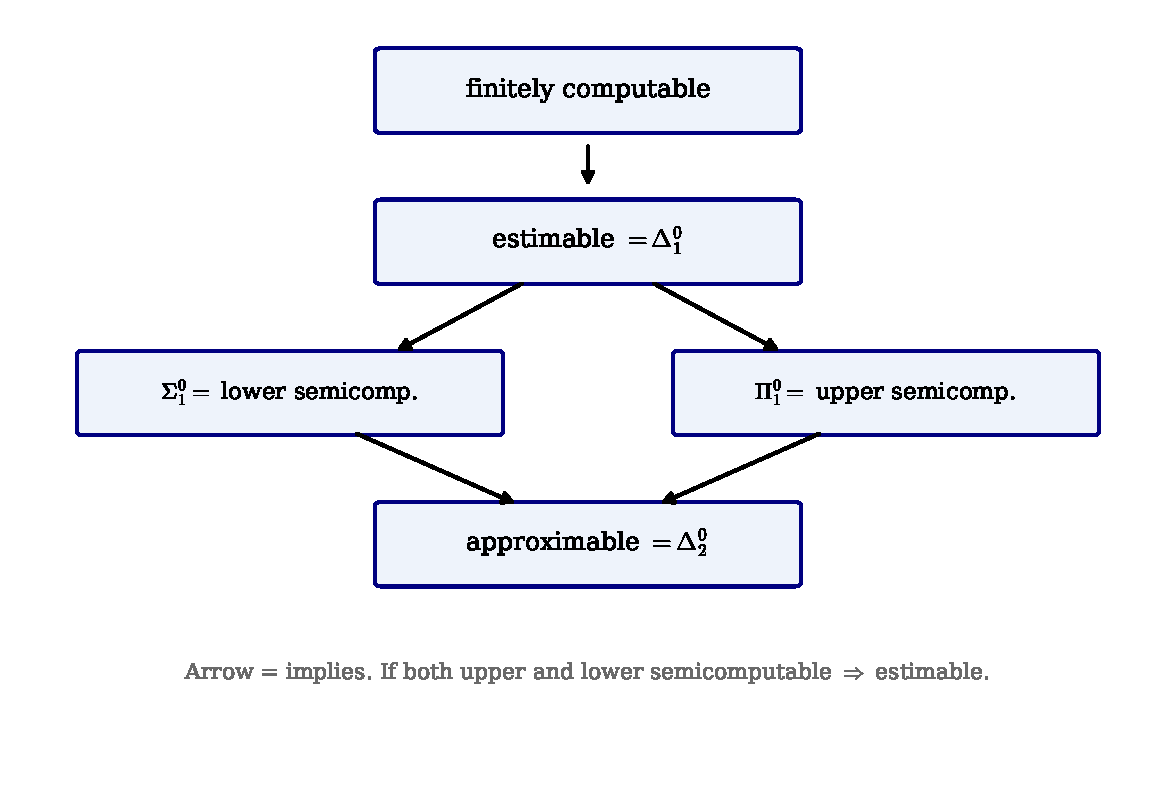
\includegraphics[width=0.46\textwidth]{implications}
  \end{block}
  \textbf{Plain English.} Reading top to bottom: finitely computable $\Rightarrow$
  estimable ($=\Delta_1^0$) $\Rightarrow$ both lower semicomputable
  ($\Sigma_1^0$) and upper semicomputable ($\Pi_1^0$) $\Rightarrow$
  approximable ($=\Delta_2^0$). Also: if $f$ is \emph{both} upper and lower
  semicomputable, then $f$ is estimable. ($\Sigma_1^0,\Pi_1^0,\Delta_1^0,\Delta_2^0$
  are labels from the arithmetic hierarchy, introduced next.) No other
  implications hold in general.
\end{frame}

% ============================================================
\begin{frame}[allowframebreaks]{Recursively Enumerable Sets We Will Meet Later}
  \begin{block}{Theorem 2.6.15 (Recursively Enumerable Sets)}
    The (countably infinite) sets $\mathcal{S}$ of (encodings of):
    \begin{enumerate}
      \item[(i)] Turing machines,
      \item[(ii)] computable partial functions,
      \item[(iii)] lower semicomputable total functions with range
        $\R \cup \{\pm\infty\}$,
      \item[(iv)] lower semicomputable semi-probability mass functions over
        $\N$ (or $\mathcal{X}^{*}$),
      \item[(v)] lower semicomputable (joint or conditional) (sequence or
        chronological) semimeasures over $\mathcal{X}^{\infty}$,
    \end{enumerate}
    are all recursively enumerable (Definition 2.6.8).
  \end{block}
  \textbf{Plain English.} This is a ``convenience catalogue'': all of these
  important classes of objects (which recur throughout the book, especially
  in the Solomonoff induction and AIXI chapters) can be effectively listed
  one by one by some master program, even though checking membership in the
  set might not be decidable.

  \framebreak
  \textbf{Proof sketch.}
  \begin{itemize}
    \item[(i)] An effective enumeration of Turing machines is easy to
      construct (list all finite binary strings and interpret each as a TM
      encoding).
    \item[(ii)] With suitable interpretation, Turing machines themselves
      describe all partial recursive functions.
    \item[(iii)] For a lower semicomputable function $f_p$ with program $p$,
      let $\varphi_p(x,t)$ be the output of the (universal machine) $U(p'x)$
      after $t$ steps, interpreted as a rational number if possible,
      otherwise $-\infty$. Then
      $\phi(x,t) := \max_{s \leq t} \varphi_p(x,s)$ is computable, monotone
      increasing, and converges to $f_p(x) = \sup_t \varphi_p(x,t)$. The set
      $\{\langle f_p \rangle : p \in \B^{*}\}$ of all such $f_p$ is exactly the
      recursively enumerable set of all lower semicomputable functions.
    \item[(iv)] Semi-probabilities additionally satisfy
      $\sum_x \varphi_p(x,t) \leq 1$. We modify the enumeration: set
      $\varphi_p(x,t) = 0$ for $x > t$ (harmless), and whenever
      $\sum_{x \leq t} \varphi_p(x,t) > 1$ (a computable check), reset
      $\varphi_p(x,t) = \varphi_p(x,t-1)$. This bounds $f_p$ to be a
      semi-probability without disturbing the $f_p$ that already were
      semi-probabilities.
    \item[(v)] Similar modifications restrict the enumeration to lower
      semicomputable (semi)measures over infinite sequences.
  \end{itemize}
  \textbf{Contrast.} The sets of \emph{computable total functions},
  \emph{computable probability mass functions}, and \emph{computable
  probability measures} are \textbf{not} recursively enumerable --- the proofs
  use diagonalization arguments similar to the halting-problem proof above.
\end{frame}

% ============================================================
\begin{frame}{Remark: Computability of Functions with Real Domain}
  \begin{block}{Remark 2.6.16 (Computability of Functions with Real Domain)}
    Defining computability for functions with continuous (real) domain is
    subtle. Most algorithms take a finite input, so they are modelled as
    functions $f : \B^{*} \to \B^{*}$. An algorithm ``computing'' the
    exponential function actually takes a (binary) fraction as input and
    outputs an approximation as a (binary) fraction. A definition of a real
    computable function $f : \R \to \R$ consistent with this
    input-approximation necessity is possible, but it renders all
    \emph{discontinuous} functions incomputable. Since the computable
    real-valued functions we encounter in this book are all benign
    (well-behaved), the intuitive understanding above is enough for our
    purposes.
  \end{block}
\end{frame}

% ============================================================
\begin{frame}[fragile]{Python: Semicomputable Sequences, Numerically}
  A numeric illustration of Definitions 2.6.11--2.6.13, using
  $f(x) = \sqrt{2} \approx 1.41421356$: we build an increasing sequence of
  rational lower bounds and a decreasing sequence of rational upper bounds,
  both converging to $f(x)$, exactly as required for lower/upper
  semicomputability.
\begin{lstlisting}
import math
true_val = math.sqrt(2)

def lower_bound(k):  return true_val - 1.0 / (k + 1)   # nondecreasing -> true_val
def upper_bound(k):  return true_val + 1.0 / (k + 1)   # nonincreasing -> true_val

for k in [1, 2, 5, 10, 100]:
    print(f"k={k:4d}  lower={lower_bound(k):.6f}  upper={upper_bound(k):.6f}")

# k=   1  lower=0.914214  upper=1.914214
# k=   5  lower=1.247547  upper=1.580880
# k= 100  lower=1.404312  upper=1.424115   (gap keeps shrinking as k grows)
\end{lstlisting}
  \textbf{Plain English.} Neither sequence alone reveals the exact value of
  $\sqrt{2}$ at any finite $k$, but each side keeps squeezing in on the truth
  --- the essence of upper/lower semicomputability.
\end{frame}

% ============================================================
\begin{frame}{Semicomputable Convergence, Visualized}
  \begin{center}
    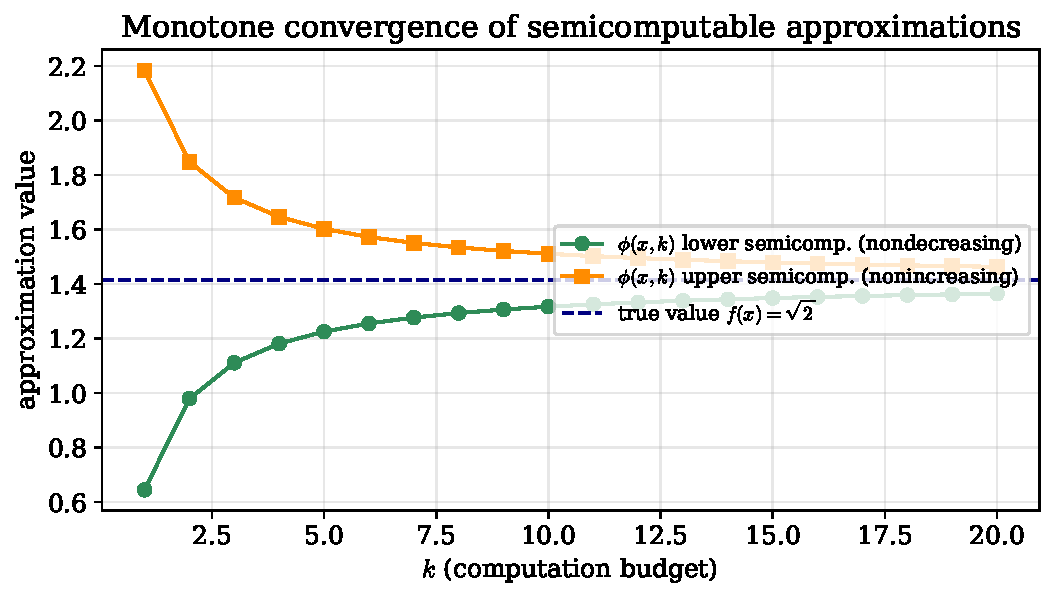
\includegraphics[width=0.62\textwidth]{semicomputable_convergence}
  \end{center}
  \textbf{Plain English.} The lower sequence (green) rises monotonically, the
  upper sequence (orange) falls monotonically, and both converge to the true
  value $\sqrt{2}$ (dashed navy line). If we additionally had a computable,
  shrinking bound on the gap $\text{upper}(k) - \text{lower}(k)$, $f$ would in
  fact be \emph{estimable} (Theorem 2.6.14) rather than merely
  semicomputable.
\end{frame}

\section{2.6.4 Arithmetic Hierarchy}

% ============================================================
\begin{frame}{Motivation: Degrees of Incomputability}
  Anything beyond ``approximable'' (Definition 2.6.13) is truly incomputable
  --- but not all incomputable problems are \emph{equally} hard. The
  \textbf{arithmetic hierarchy} classifies problems by \emph{degrees of
  incomputability}, using \textbf{quantifiers} (or, equivalently, access to a
  hypothetical \emph{halting oracle}, a device that can magically answer
  halting-problem queries).

  \vspace{2mm}
  \textbf{Intuition.} At the base of the hierarchy sit problems solvable by
  elementary algorithms with no quantifiers at all (e.g.\ checking the parity
  of a number) --- these are the ordinary computable problems. Moving up each
  tier of the hierarchy requires one additional layer of alternating
  quantifiers (``for all,'' ``there exists'') to state the problem.
\end{frame}

% ============================================================
\begin{frame}{Definition: The Arithmetic Hierarchy $\Sigma_n^0, \Pi_n^0, \Delta_n^0$}
  \begin{block}{Definition 2.6.17 (Arithmetic Hierarchy)}
    A set $A \subseteq \N_0$ is $\Sigma_n^0$ if and only if there is a
    computable relation $\eta$ such that
    \[
      k_0 \in A \iff \exists k_1 . \forall k_2 \dots Q_n k_n . \; \eta(k_0,k_1,k_2,\dots,k_n)
    \]
    where $Q_n = \forall$ if $n$ is even and $Q_n = \exists$ if $n$ is odd.
    Similarly, $A$ is $\Pi_n^0$ if the outer-most quantifier is $\forall k_1$
    instead. Furthermore,
    \[
      A \subseteq \N_0 \text{ is } \Pi_n^0 \iff \N_0 \setminus A \text{ is } \Sigma_n^0, \qquad
      A \subseteq \N_0 \text{ is } \Delta_n^0 \iff A \text{ is both } \Sigma_n^0 \text{ and } \Pi_n^0.
    \]
  \end{block}
  \textbf{Plain English, piece by piece.} $\eta$ (eta) is an ordinary,
  fully computable yes/no test on a tuple of numbers. $\exists k_1$ means
  ``there exists some $k_1$ making this true''; $\forall k_2$ means ``for
  every $k_2$, this holds.'' $\Sigma_n^0$ (sigma) means: the membership test
  for $A$ can be phrased using $n$ alternating quantifiers, starting with
  $\exists$. $\Pi_n^0$ (pi) is the mirror image, starting with $\forall$.
  $\Delta_n^0$ (delta) means the set can be phrased \emph{both} ways --- it
  sits in the intersection, and is ``as easy as'' both perspectives suggest.
  The subscript $n$ counts how many quantifier layers are needed: the more
  layers, the higher up (and harder) in the hierarchy.
\end{frame}

% ============================================================
\begin{frame}{The Hierarchy is a Strict Chain of Inclusions}
  We can think of $\Sigma_n^0$ and $\Pi_n^0$ as an increasing hierarchy of
  complexity, where $n$ counts the number of alternating quantifiers needed
  to describe $A$ in first-order logic, together with a computable relation
  $\eta$. Instead of $A \subseteq \N_0$, we may equally allow
  $A \subseteq \B^{*}$, using an effective binary encoding of objects
  (including tuples); and indeed any recursive set sits at the very bottom
  (membership is decidable, i.e.\ the indicator function is computable). The
  ``$0$'' superscript in $\Sigma^0$ signals that there are even higher
  hierarchies (e.g.\ the \emph{analytic hierarchy} $\Sigma_n^1$, higher-order
  arithmetic whose lowest member $\Sigma_0^1$ contains, in a certain sense,
  the whole arithmetic hierarchy $\cup_n \Sigma_n^0$).
\end{frame}

% ============================================================
\begin{frame}{The Arithmetic Hierarchy, Visualized}
  \begin{center}
    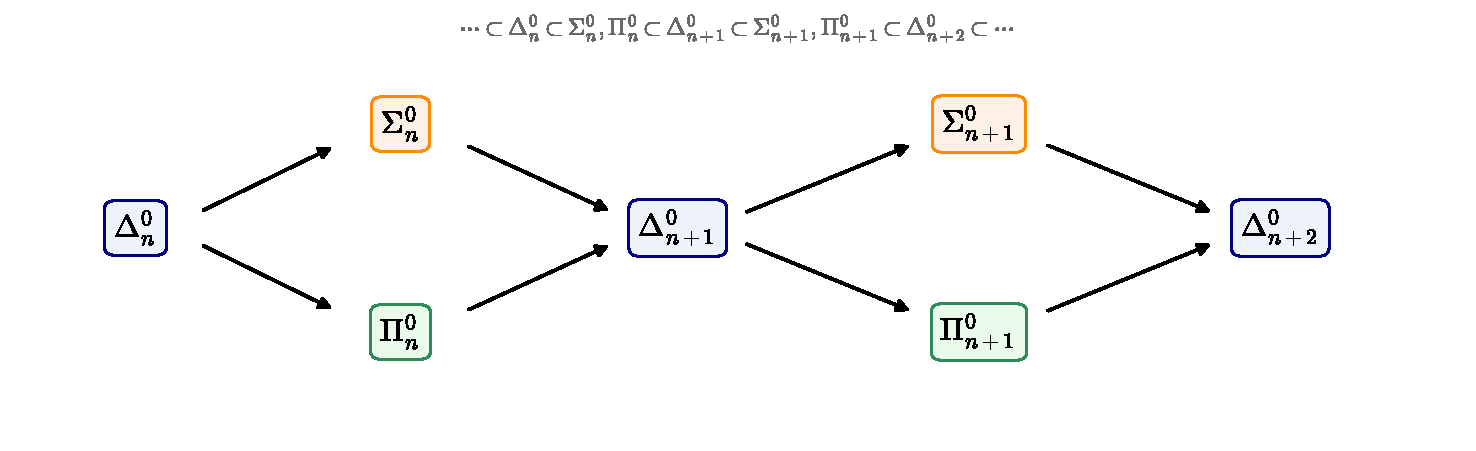
\includegraphics[width=0.85\textwidth]{arithmetic_hierarchy}
  \end{center}
  \textbf{Plain English.} Each arrow is a strict subset relation ($\subset$):
  every set at one tier is contained in (but not equal to) the sets one tier
  higher. The hierarchy never collapses --- there are always strictly harder
  problems further up.
\end{frame}

% ============================================================
\begin{frame}{Extending the Hierarchy to Functions: $\Sigma/\Pi/\Delta$-Functions}
  \begin{block}{Definition 2.6.18 ($\Sigma/\Pi/\Delta$-Functions)}
    A function $f : \B^{*} \to \R$ is called $\Sigma_n^0$ (or $\Pi_n^0$, or
    $\Delta_n^0$) if and only if the set
    $I_f := \{(x,q) \in \B^{*} \times \Q : q < f(x)\}$ is $\Sigma_n^0$ (or
    $\Pi_n^0$, or $\Delta_n^0$ respectively). That is, given an enumeration
    $g : \B^{*} \times \Q \to \N_0$, the image $g(I_f) \in \Sigma_n^0$ (or
    $\Pi_n^0$, or $\Delta_n^0$).
  \end{block}
  \textbf{Plain English.} $I_f$ (the ``strictly-below-graph'' set) collects
  every pair (input $x$, rational threshold $q$) for which the function value
  $f(x)$ exceeds $q$. Classifying $f$ in the hierarchy is done by classifying
  \emph{this associated set} of (input, threshold) pairs, using an
  enumeration $g$ that turns pairs into single natural numbers so
  Definition 2.6.17 applies directly.

  \vspace{2mm}
  \textbf{Reconnecting to earlier definitions.} Theorem 2.6.14's four notions
  are exactly the lowest rungs of this ladder: \textbf{estimable} functions
  are $\Delta_1^0$, \textbf{lower semicomputable} functions are $\Sigma_1^0$,
  \textbf{upper semicomputable} functions are $\Pi_1^0$, and
  \textbf{approximable} functions are $\Delta_2^0$. Note also a subtlety: for
  $f \in \Delta_n^0$, we have $\{(x,y) : f(x) > g(y)\} \in \Sigma_n^0$, but
  $\{(x,y) : f(x) \leq g(y)\} \in \Pi_n^0$ (the ``$=$'' boundary case is what
  causes the asymmetry).
\end{frame}

% ============================================================
\begin{frame}[allowframebreaks]{Properties of $\Sigma/\Pi/\Delta$-Functions}
  \begin{block}{Theorem 2.6.19 (Properties of $\Sigma/\Pi/\Delta$-Functions)}
    \begin{enumerate}
      \item[(i)] $\Sigma_n^0 = -\Pi_n^0$ \quad ($f \in \Sigma_n^0 \iff -f \in \Pi_n^0$)
      \item[(ii)] $\Delta_m^0(\Delta_n^0) = \Delta_{n+m-1}^0$ (function
        concatenation), esp.\ $f(\Delta_n^0) \subseteq \Delta_n^0$ for
        $f \in \Delta_1^0$
      \item[(iii)] $\Delta_m^0(\Sigma_n^0) = \Delta_{n+m}^0$ and
        $\Delta_m^0(\Pi_n^0) = \Delta_{n+m}^0$
      \item[(iv)] $\sup \Delta_n^0 = \sup \Sigma_n^0 = \Sigma_n^0$, \quad
        $\inf \Delta_n^0 = \inf \Pi_n^0 = \Pi_n^0$, \quad
        $\sup \Pi_n^0 = \Sigma_{n+1}^0$, \quad $\inf \Sigma_n^0 = \Pi_{n+1}^0$
      \item[(v)] $\limsup_t = \inf_s \sup_{t \geq s}$ and
        $\liminf_t = \sup_s \inf_{t \geq s}$, hence e.g.
        $\lim \Delta_n^0 = \Delta_{n+1}^0$
      \item[(vi)] $f(\Sigma_n^0) \subseteq \Sigma_n^0$ for monotone increasing
        $f \in \Sigma_1^0$
      \item[(vii)] $f(\Pi_n^0) \subseteq \Pi_n^0$ for monotone increasing
        $f \in \Pi_1^0$
      \item[(viii)] $+, \times, \exp, \log, \dots \in \Delta_1^0$ and finite
        $\max, \min, \sum \in \Delta_1^0$, all monotone increasing
      \item[(ix)] $\sum^{\infty} = \lim_t \sum^t$ in general, hence
        $\sum^{\infty} \Delta_n^0 = \Delta_{n+1}^0$ in general
      \item[(x)] $\sum^{\infty} = \sup_t \sum^t$ if applied to non-negative
        functions, hence $\sum^{\infty} \Sigma_n^{0+} = \Sigma_n^{0+}$.
    \end{enumerate}
  \end{block}

  \framebreak
  \textbf{Plain English --- why this list matters in practice.} These ten
  rules are a ``calculus'' for the arithmetic hierarchy: given the
  classification of some building-block functions, you can often read off
  (at least an upper bound on) the degree of incomputability of a
  \emph{composite} function directly from its formula, without redoing a
  diagonalization-style proof from scratch every time.

  \begin{itemize}
    \item (i) says $\Sigma$ and $\Pi$ are mirror images under negation ---
      classifying $f$ from below is the same difficulty as classifying $-f$
      from above.
    \item (ii)--(iii) say that composing/combining $\Sigma,\Pi,\Delta$
      functions moves you up the hierarchy by an amount you can predict just
      by adding indices --- composing a $\Delta_1^0$ (estimable) function with
      a $\Delta_n^0$ function stays at $\Delta_n^0$: applying computable
      post-processing to a computable quantity costs nothing.
    \item (iv)--(v) say that taking suprema, infima, or limits of families
      of $\Sigma_n^0/\Pi_n^0/\Delta_n^0$ functions moves you up the hierarchy
      by exactly one level in a predictable direction: $\sup$ pushes toward
      $\Sigma$, $\inf$ pushes toward $\Pi$.
    \item (vi)--(vii) say monotone transformations by an already-classified
      monotone function do not increase the hierarchy level.
    \item (viii) is a convenience list: ordinary arithmetic
      ($+,\times,\exp,\log$) and finite max/min/sums are all as easy as
      possible ($\Delta_1^0$, i.e.\ estimable).
    \item (ix)--(x) distinguish infinite sums in general (one level up, since
      an infinite sum is a limit of partial sums) from infinite sums of
      \emph{non-negative} terms specifically (no level increase, since a
      non-negative sum is simply a supremum of partial sums, which for
      $\Sigma^{0+}$, i.e.\ non-negative $\Sigma_n^0$ functions, stays in
      $\Sigma_n^{0+}$ by rule (iv)).
  \end{itemize}
\end{frame}

% ============================================================
\begin{frame}[fragile]{Python: Deciding a $\Sigma_1^0$ Predicate by Bounded Search}
  A $\Sigma_1^0$ statement is $\exists k_1 . \eta(k_0,k_1)$ for a computable
  $\eta$ --- only \emph{semi}-decidable in general: ``yes'' is certified by
  finding a witness, but ``no'' may need an unbounded search. Here
  $\eta(n,d)$ tests whether $d$ divides $n$ nontrivially; ``$n$ is
  composite'' $= \exists d . \eta(n,d)$, with a witness search bounded by
  $\sqrt{n}$, so it is in fact fully decidable ($\Delta_1^0$).
\begin{lstlisting}
def eta(n, d):  return 1 < d < n and n % d == 0   # computable relation

def is_composite(n):                      # exists d . eta(n,d), bounded by sqrt(n)
    for d in range(2, int(n**0.5) + 2):
        if eta(n, d):
            return True, d                # witness found
    return False, None

for n in [7, 12, 17, 91]:
    composite, witness = is_composite(n)
    print(f"n={n:3d}: composite(d={witness})" if composite else f"n={n:3d}: prime")

# n=  7: prime          n= 12: composite(d=2)
# n= 17: prime          n= 91: composite(d=7)
\end{lstlisting}
  \textbf{Plain English.} A witness $d$ certifies membership immediately
  ($\exists$); knowing the search bound $\sqrt{n}$ upgrades this from merely
  semi-decidable to fully decidable. Without a bound (e.g.\ ``does program
  $M$ ever output $7$?''), the search could run forever --- the
  semi-decidable character of a general $\Sigma_1^0$ set.
\end{frame}

% ============================================================
\begin{frame}{Summary: Section 2.6}
  \begin{itemize}
    \item An \textbf{algorithm} is formalized by a \textbf{Turing machine}
      (Definition 2.6.2): finite control + infinite tape. The
      \textbf{Church--Turing thesis} asserts this captures every intuitive
      notion of ``computable by a fixed procedure,'' and is corroborated by
      the equivalence of lambda calculus, general recursive functions, and
      many other \textbf{Turing complete} systems.
    \item The \textbf{Halting Problem} (Theorem 2.6.7) is the canonical
      undecidable problem: no Turing machine can always correctly decide
      whether another halts, proved by a self-referential diagonalization
      argument descending from Gödel's incompleteness theorem.
    \item Real-valued functions admit graded notions of computability:
      \textbf{finitely computable} $\Rightarrow$ \textbf{estimable}
      ($\Delta_1^0$) $\Rightarrow$ \textbf{lower} ($\Sigma_1^0$) /
      \textbf{upper} ($\Pi_1^0$) \textbf{semicomputable} $\Rightarrow$
      \textbf{approximable} ($\Delta_2^0$) (Theorem 2.6.14).
    \item The \textbf{arithmetic hierarchy} $\Sigma_n^0, \Pi_n^0, \Delta_n^0$
      (Definition 2.6.17) grades incomputable problems by the number of
      alternating quantifiers needed to state them, extends to real-valued
      functions (Definition 2.6.18), and obeys a rich algebra of closure
      properties (Theorem 2.6.19) that lets us classify composite functions
      without re-deriving everything from scratch.
    \item These graded notions of computability will recur throughout the
      book, especially when discussing Kolmogorov complexity, Solomonoff's
      universal distribution, and the (in general incomputable) AIXI agent.
  \end{itemize}
\end{frame}

\end{document}
